\chapter{Testing}\label{sec:testing}

In this chapter, we discuss the testing strategy and the test results for the final version of \texttt{JHygge}.
There are two parts to testing \texttt{JHygge}; one is a functionality test to validate requirement stated in \ref{sec:requirements},
and the other is an end-user test, where the end-user is a current or former student of the course ``02247 - Compiler Construction''
is asked to implement a simple extension to the hygge language in \texttt{JHygge} and provide feedback about their experience.

\section{Functionality testing of \texttt{JHygge}}

For testing the functionality of the new \texttt{JHygge} compiler, a test suite akin to that of \texttt{hyggec} has be made.
Here, hygge source files for testing are placed in folders marked for testing. These folders are divided first by compiler
stage/phase and subsequently by whether the program should pass or fail the test. One thing to note is that the test
for the code generation phase will only check that the test program compiles, but not whether it runs correctly as the
test code does not invoke the JVM on the compiled bytecode.

In addition to the automated test suite, a lot of manual testing of each compiler phase has been done during prototyping.
In this endevour, the \texttt{JHygge} CLI made using the \texttt{PicoCLI}-framework proved to valuable as it provides a
quick and easy-to-use interface with access to each individual compiler phase with a single command.

\section{End-user testing of \texttt{JHygge}}

For the end-user test, current and former students are given a task to implement a simple language feature in \texttt{JHygge}:
a subtraction operator for numerical values. The students are presented with eight subtasks in which they set up the compiler
project and toolchain and subsequently implement the subtraction operator at the different stages of the compiler. After
each task, the student is asked to describe their experience implementing the particular stage in \texttt{JHygge}. For the
final question, the student is asked to give their closing remarks. On figure \ref{fig:end_user_test}, the form with subtasks
that was shared with current and former students of the compiler construction course is shown.

\begin{figure}[H]
\centering
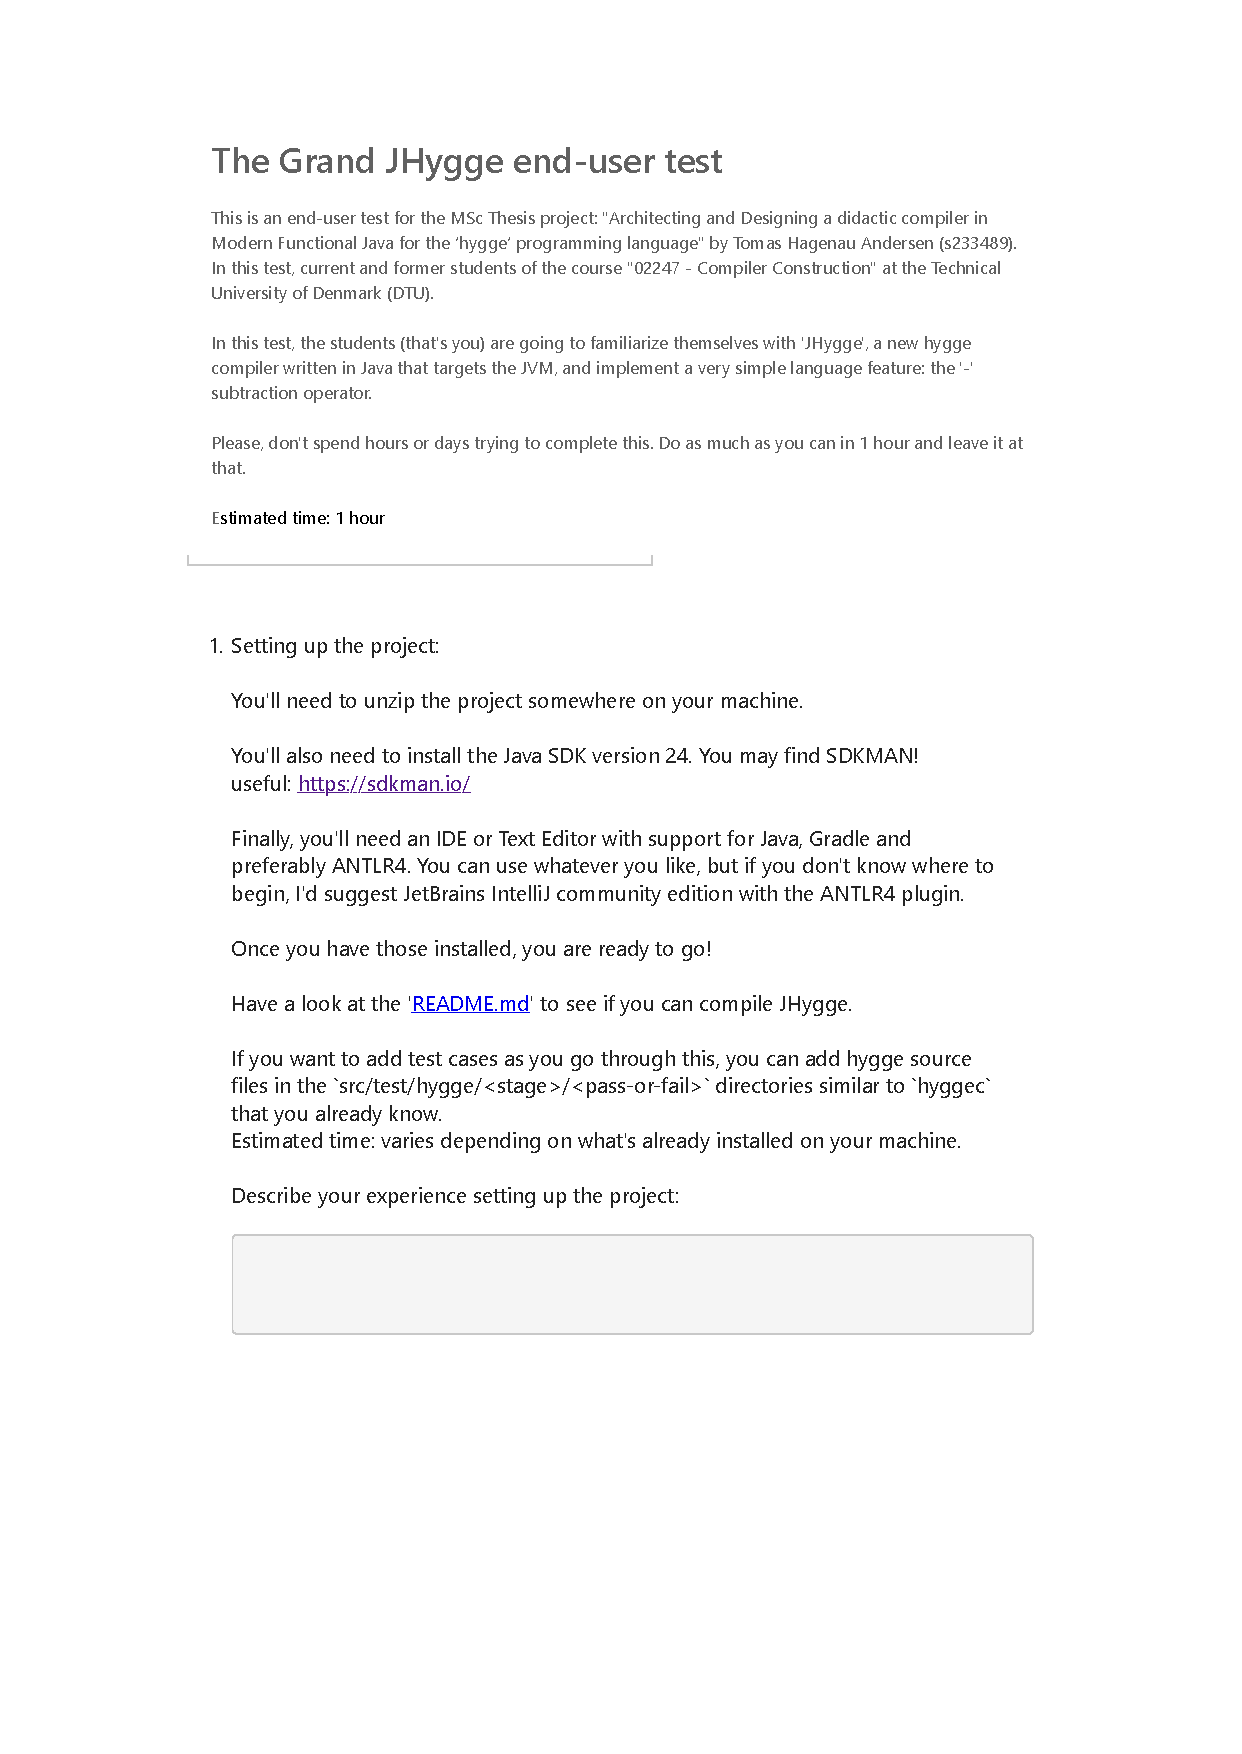
\includegraphics[width=0.3\textwidth]{Pictures/the_grand_jhygge_end_user_test.pdf}
\caption{The questionaire for the end-user test handed out to students}
\label{fig:end_user_test}
\end{figure}

The end-user test ran from May 28th to June 18th 2025. During this period, the students had finished the course ``02247 - Compiler Construction'',
so they should have been available although some may have chosen to take a course in the 3-week period in June.

Unfortunately, none of the more than 200 students chose to participate in the end-user test, meaning that we do not have any test results
to present despite our efforts. Therefore, we cannot say anything conclusive about the user-friendliness of the new \texttt{JHygge} compiler
nor can we in any reasonable way compare it to the user-friendliness of the existing \texttt{hyggec} compiler.
